% from
% 2012__Stefan_Lukits__The_Principle_of_Maximum_Entropy_and_a_Problem_in_Probability_Kinematics__PSA_version.tex:
% This is an edited version of
% 2011__Stefan_Lukits__The_Principle_of_Maximum_Entropy_and_a_Problem_in_Probability_Kinematics.tex
% Some interesting material from the 2011 file is missing, because we
% had to reduce the word count. On the other hand, the information is
% condensed, improved, and there is some additional material on Halpern
% and Gruenwald's CAR. I would run a diff and scan the relevant sections
% of the 2011 file to see the missing paragraphs, but use this one for
% further projects.

\documentclass[12pt]{article}

\setlength{\marginparwidth}{1.2in}
\let\oldmarginpar\marginpar
\renewcommand\marginpar[1]{\-\oldmarginpar[\raggedleft\footnotesize #1]%
{\raggedright\footnotesize #1}}

\frenchspacing % no extra space at the end of a sentence

\setlength{\parindent}{0in}
\setlength{\parskip}{.1in}

\raggedbottom

%\pagestyle{empty}

% 	PACKAGES
% \usepackage[small,bf]{caption}
% \let\bcode\textbgreek
% \usepackage[bgreek,english]{babel}
% \usepackage{setspace}
\usepackage{amsfonts}
\usepackage{amssymb}
\usepackage{amsmath}
% \usepackage{german}
% \usepackage{hebtex}
\usepackage{graphicx}
% \usepackage[german]{babel}
% \usepackage{endnotes}
% \let\footnote=\endnote
% \usepackage{rotating}
\usepackage{enumerate}

\newcommand{\kapt}[1]{\textbf{{\thechap}. #1}\addtocounter{chap}{1}}
\newcommand{\nootag}{}

\newcommand{\tbd}[1]{}
\newcommand{\qnull}[1]{`#1'}
\newcommand{\qeins}[1]{``#1''}
\newcommand{\qzwei}[1]{`#1'}
\newcommand{\erf}[0]{\mbox{erf}}
\newcommand{\anum}[0]{a'}
\newcommand{\bnum}[0]{b'}
\newcommand{\cnum}[0]{c'}
\newcommand{\hnum}[0]{h'}
\newcommand{\knum}[0]{k'}
\newcommand{\wnum}[0]{w'}
\newcommand{\aden}[0]{a''}
\newcommand{\bden}[0]{b''}
\newcommand{\cden}[0]{c''}
\newcommand{\hden}[0]{h''}
\newcommand{\kden}[0]{k''}
\newcommand{\wden}[0]{w''}
\def\lwv{.6}

\newif\ifNumericalOrYear
\NumericalOrYeartrue
% \NumericalOrYearfalse
\ifNumericalOrYear
\usepackage[numbers,colon]{natbib}
\else
\usepackage[round,colon]{natbib}
\fi
\newif\ifPageP
\PagePtrue
% \PagePfalse
\ifPageP
\newcommand{\PageP}{p.~}
\else
\newcommand{\PageP}{}
\fi

\newcommand{\scite}[3]{\ifnum#1=1\ifNumericalOrYear\citep{#2}\else\citeyearpar{#2}\fi\else
\ifnum#1=2\ifNumericalOrYear\citep[#3]{#2}\else\citep[{\PageP}#3]{#2}\fi\else
\ifnum#1=3\ifNumericalOrYear(\citet[#3]{#2})\else\citep[{\PageP}#3]{#2}\fi\else
\ifnum#1=4\ifNumericalOrYear\citet{#2}\else\citet{#2}\fi\else
\ifnum#1=5\ifNumericalOrYear(\citet{#2})\else\citep{#2}\fi\else
\ifnum#1=6\ifNumericalOrYear(\citet[#3]{#2})\else\citep[{\PageP}#3]{#2}\fi\else
\ifnum#1=7\ifNumericalOrYear\citep{#2}\else\citealp{#2}\fi\else
\ifnum#1=8\ifNumericalOrYear\citep[#3]{#2}\else\citealp[{\PageP}#3]{#2}\fi\else
\textbf{[invalid scite code]}\fi\fi\fi\fi\fi\fi\fi\fi}

\newenvironment{quotex}{\begin{quote}\begin{footnotesize}}{\end{footnotesize}\end{quote}}
% \newenvironment{quotex}{\begin{quote}\begin{footnotesize}\begin{singlespace}}{\end{singlespace}\end{footnotesize}\end{quote}}

\begin{document}

\title{The Principle of Maximum Entropy and a Problem in Probability Kinematics}

\author{Stefan Lukits}

\maketitle

\newcounter{chap}

\setcounter{chap}{1}

\begin{quotex}
  Acknowledgments: Thanks to James Baugh at the Mathematics Department
  at GCSU in Milledgeville, GA, for helping me when I was stuck with
  an integral. Somebody hiding behind the pseudonym micromass helped
  me with a binomial identity on physicsforums.com. Thanks to
  Jan-Willem Romeijn, Adom Giffin, and Paul Bartha for comments in
  writing and the many verbal comments from participants at the 2011
  meeting of the Canadian Society for the History and Philosophy of
  Science in Fredericton, NS.
\end{quotex}

\kapt{Introduction}

There are cases in which, given evidence, we cannot use Bayes' formula
to deliver a set of posterior probabilities given a set of prior
probabilities. The Bayesian method presupposes that evidence comes in
the form of an event. As Jeffrey observed, however, the evidence may
not relate the certainty of an event but a reassessment of its
uncertainty or its probabilistic relation to other events (see
\scite{8}{jeffrey65}{153ff}), expressible in a shift in expectation
(see \scite{7}{hobson71}{}). Bas van Fraassen has come up with a good
example from the 1980 comedy film \emph{Private Benjamin} (see
\scite{7}{fraassen81}{}), in which Goldie Hawn portrays a
Jewish-American woman (Judy Benjamin) who joins the U.S. Army.

\begin{figure}[h]
  \begin{flushright}
    \begin{minipage}[h]{.8\linewidth}
      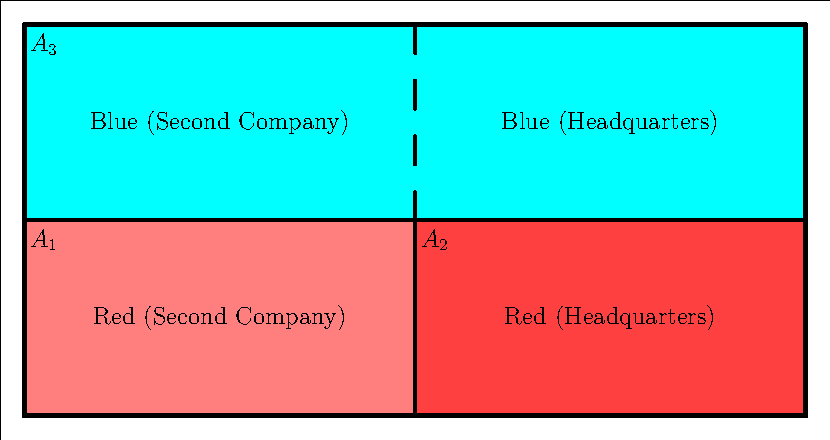
\includegraphics[width=\textwidth]{judy.pdf}
      \caption{Judy Benjamin's map. Blue territory ($A_{3}$) is friendly and
        does not need to be divided into a Headquarters and a Second
        Company area.}
      \label{fig:map}
    \end{minipage}
  \end{flushright}
\end{figure}

In the movie, Judy Benjamin is on an assignment and lands in a place
where she is not sure of her location. She is on team Blue. Because of
the map, her probability of being in Blue territory equals the
probability of being in Red territory, and being in the Red Second
Company area equals the probability of being in the Red Headquarters
area. Her commanders inform Judy by radio that in case she is in Red
territory, her chance of being in their Headquarters area is three
times the chance of being in their Second Company area.

There is no immediately obvious event space in which we can condition
on an event $E$. Grove and Halpern \scite{1}{grovehalpern97}{} have
written an article on how to construct such event spaces and then
condition on the event that Judy Benjamin receives the information
that she receives from her commanders. They admit, however, that the
construction of such spaces (sometimes called retrospective
conditioning) is an exercise in filling in missing details and
supplying information not contained in the original problem.

Largely in the field of physical statistics (but also in others, for
an impressive (and outdated) list see \scite{8}{shorejohnson80}{26}),
problems like the Judy Benjamin problem occur frequently and are
usually solved using the principle of maximum entropy, \textsc{maxent}
from now on. The constraint imposed by the evidence transforms
the prior probability distribution in a way that secures minimal
information gain. We want a posterior probability distribution that
reflects the evidence but does not provide more information than
necessary. If the prior probability distribution is uniform, this
principle is called the principle of maximum entropy; if it is not
uniform, it is also called the infomin principle, the principle of
minimal discrimination, or the principle of minimum cross-entropy. The
mathematics leading to the solution of these types of problems is
elegant and has compelling properties, outlined in a seminal article
by John E. Shore and Rodney W. Johnson \scite{1}{shorejohnson80}{}.

Indulging for a moment in an artificial contrast, philosophers, as
opposed to physicists, are generally skeptical about the objectivism
implied by \textsc{maxent}. E.T. Jaynes, the father of the principle,
sought to provide a uniquely admissible probability function given a
particular knowledge state. For many philosophers, this approach is
excessively aprioristic (see \scite{8}{seidenfeld79}{414}), violates
intuitions (see \scite{7}{grovehalpern97}{}), and does not do justice
to the thought a human inquirer (not a machine) needs to put into a
scenario in order to solve it intelligently. I shall call the last
principle the full employment theorem, leaning on a theorem in
computer science that states that a human programmer is necessary to
write optimal programs. 

Joseph Halpern writes in his recent book \emph{Reasoning About
  Uncertainty} that \qeins{there is no escaping the need to understand
  the details of the application} \scite{2}{halpern03}{423} and
concludes that \textsc{maxent} is a valuable tool, but should be used
with care (see \scite{8}{grovehalpern97}{110}), explicitly basing his
remark on the counterintuitive behaviour of the Judy Benjamin problem.
Diaconis and Zabell state \qeins{that any claims to the effect that
  maximum-entropy revision is the only correct route to probability
  revision should be viewed with considerable caution}
\scite{2}{diaconiszabell82}{829}. \qeins{Great caution}
\scite{2}{howsonfranklin94}{456} is also what Colin Howson and Allan
Franklin advise about the claim that the posterior probabilities
provided by \textsc{maxent} are as like the prior probabilities as it
is possible to be given the constraints imposed by the data.

Grove and Halpern, in their article about the Judy Benjamin problem,
admonish the objectivists in accordance with the full employment
theorem that \qeins{one must always think carefully about precisely
  what the information means} \scite{2}{grovehalpern97}{6}, and
\qeins{the only right way to update, especially in an incompletely
  specified situation, is to think very carefully about the real
  nature and origin of the information we receive}
\scite{2}{grovehalpern97}{3}. Igor Douven and Jan-Willem Romeijn
advocate an innovative approach to the Judy Benjamin problem, in which
epistemic entrenchment supplies a subjectivist perspective on these
types of problem and delivers a Jeffrey partition so that instead of
\textsc{maxent} Jeffrey's rule can be applied. They agree with Bradley
that \qeins{even Bayes' rule \qzwei{should not be thought of as a
    universal and mechanical rule of updating, but as a technique to
    be applied in the right circumstances, as a tool in what Jeffrey
    terms \emph{the art of judgment}.} In the same way, determining
  and adapting the weights [epistemic entrenchment] supposes, or
  deciding when Adams conditioning applies, may be an art, or a skill,
  rather than a matter of calculation or derivation from more
  fundamental epistemic principles} \scite{2}{douvenromeijn09}{16}
(for the Bradley quote see \scite{8}{bradley05}{362}).

Teddy Seidenfeld gives his own reasons why he is not an objective
Bayesian in an article entitled \qeins{Why I Am Not an Objective
  Bayesian} \scite{1}{seidenfeld79}{} (claiming that in particular
circumstances involving noise factors \textsc{maxent} will
inappropriately provide more information based on less evidence). Jos
Uffink targets especially Shore and Johnson's assumptions when they
identify \textsc{maxent} as the unique method of determining posterior
probability distributions, given certain types of constraints. Uffink
shows how a more reasonable restatement of Shore and Johnson's
assumptions results in a whole class of updating procedures, the
so-called R{\'e}nyi entropies (see \scite{7}{uffink95}{}), affirming
Carnap's conjecture that there is a continuum of updating procedures
rather than one that is unique. This also appears to be van Fraassen's
conclusion when he suggests that \textsc{maxent} is a special instance
of a family of principles which are consistent relative to specified
assumptions (see \scite{7}{fraassenetal86}{}). Dias and Shimony
provide a very interesting case of failure for \textsc{maxent} that we
will not address in this paper because it is not relevant to the
Judy Benjamin problem (see \scite{7}{diasshimony81}{}), although we
hope to address it at a later date.

There are attempts, with the help of Lagrange multipliers, to show
that \textsc{maxent} is a generalization of Jeffrey's rule, which
itself is a generalization of Bayesian conditionalization. The domains
of these updating rules are affine constraints for \textsc{maxent}
(these are most general and include cases in which Bayesian
conditionalization and Jeffrey's rule can be applied, for a
mathematical definition of affine constraints see
\scite{7}{csiszar67}{}, the useful summary in
\scite{8}{howsonfranklin94}{456} or in \scite{8}{williams80}{136ff});
proper probability kinematics in Jeffrey's sense for Jeffrey's rule,
where evidence changes the probability of a partition of the event
space; and events with prior probabilities for Bayesion
conditionalization, respectively. There is, however, a debate whether
\textsc{maxent} is in peaceful coexistence with, is in conflict with,
or is a generalization of Bayesian conditionalization (see
\scite{7}{uffink96}{}). For examples where \textsc{maxent}, Jeffrey's
rule, and Bayesian conditionalization disagree see
\scite{7}{williamson09}{}. Brian Skyrms advocates in
\scite{1}{skyrms85}{} that, in the opposite direction, Bayesian
conditionalization is a generalization of \textsc{maxent}.

Resistance to these relativizing tendencies on the part of the full
employment camp in philosophy mostly comes from physical statistics,
where much effort has gone into showing the consistency of
\textsc{maxent} and Bayesian updating (see
\scite{7}{catichagiffin06}{}), and where the family of R{\'e}nyi
functions proposed by Uffink are ruled out (see
\scite{7}{giffin08}{}). Adom Giffin seeks to \qeins{show that
  \textsc{maxent} is capable of producing every aspect of orthodox
  Bayesian inference and [to] prove the complete compatibility of
  Bayesian and entropy methods} (in the abstract of
\scite{7}{giffin08}{}). Jon Williamson wants to demonstrate that in
all cases where objectivist methods disagree with Bayesian
conditionalization, objectivist methods like \textsc{maxent} prevail
(see \scite{7}{williamson09}{}).

What is lacking in the literature is an explanation by \textsc{maxent}
advocates of the counter-intuitive behaviour of the cases repeatedly
quoted by the relativizers. This is especially surprising as we are
not dealing with an array of counter-examples but only a handful, the
Judy Benjamin problem (and the Dias-Shimony objection) being prime
among them. In Halpern's textbook, for example, the reasoning is as
follows: \textsc{maxent} is a promising candidate delivering unique
posterior probability distributions; but, unfortunately, there is
counter-intuitive behaviour in one specific case, the Judy Benjamin
case (see \scite{8}{halpern03}{})\tbd{provide reference}; therefore,
we must abide by the eclectic principle of considering not only
\textsc{maxent}, but also lower and upper probabilities,
Dempster-Shafer belief functions, possibility measures, ranking
functions, relative likelihoods, and so forth. The human inquirer is
the final arbiter between these conditionalization methods.

The goal of this paper is to undermine the notion that
\textsc{maxent}'s suggested solution for the Judy Benjamin problem is
counter-intuitive. Therefore, Halpern does not give us sufficient
grounds for the eclecticism, or full employment, that he advocates. On
the contrary, we will show that another intuitive approach, the
powerset approach, lends significant support to the solution provided
by \textsc{maxent} for the Judy Benjamin problem. Our argument is
vaguely related to Jaynes' use of the Wallis derivation to justify
\textsc{maxent} in \scite{8}{jaynes98}{351ff}. The intuition that
\textsc{maxent}'s solution for the Judy Benjamin problem violates (we
will call it T1) is based on fallacious independence and uniformity
assumptions. There is another powerful intuition (we will call it T2)
in direct contradiction to T1 which \textsc{maxent} obeys.

Probability kinematics resembles ethics in the sense that there are
all kinds of things we are able to say about the relations between our
intuitions and the prescriptions or rules we propose. We never cease
to be vulnerable, however, to the question why the states of affairs
we describe should entail that we have one set of probability
assignments and updating strategies and not another. That an
observation or a piece of evidence should change our assessment of
uncertainty with respect to relevant propositions and events in
particular ways cannot be a matter of logical consistency. Even a
Dutch Book argument rests on assumptions that are entangled with the
relations and intuitions we are supposed to explain.

Admitting the voluntarist nature of our adherence to updating rules or
updating constraints, we never lose a sense of need for what ethicists
in Rawl's tradition call a reflective equilibrium. It is not the
intuitions about particular cases alone, nor the general judgments
they sometimes inspire, that carry away the prize, but rather a
balance between them. The principle of maximum entropy is a poster
child for this method: it is a principle with great generality and
scope, arguably outperforming all others, but it also raises worries
in particular cases. There is beauty in the fact that, as sweeping as
the principle is, it cannot accommodate everything we think and feel
about how probability kinematics should proceed.

This paper cautions, however, against undue enthusiasm about the full
employment theorem, the view that ultimately all rules and methods of
conditionalization are tools in the hand of a human inquirer,
expressing that which one to use must always be based on the
intuitive, intelligent, and creative labour of the user. Probability
kinematics is not a sit-down dinner: various approaches mingle, easily
shift positions, and have access to the buffet table from different
angles. There is no Archimedean position even for the view that, when
all is said and done, a special place of arbitration remains for the
art of human inquiry.

\kapt{Two Intuitions}

There are two pieces of information relevant to Judy Benjamin when she
decides on her posterior probability assignment. We will call them
({\ref{eq:map}}) and ({\ref{eq:hdq}}). As in figure~\ref{fig:map},
$A_{1}$ is Red's Second Company area, $A_{2}$ is Red's Headquarters
area, $A_{3}$ is Blue territory. Judy presumably wants to be in Blue
territory, but if she is in Red territory, she would prefer their
Second Company area (where enemy soldiers are not as well-trained as
in the Headquarters area).

\begin{enumerate}
\item[({\ref{eq:map}})] Judy has no idea where she is. She is on team Blue.
  Because of the map, her probability of being in Blue territory
  equals the probability of being in Red territory, and being in the Red
  Second Company area equals the probability of being in the Red
  Headquarters area.
\item[({\ref{eq:hdq}})] Her commanders inform Judy that in case she is in Red
  territory, her chance of being in their Headquarters area is three
  times the chance of being in their Second Company area.
\end{enumerate}

In formal terms (sloppily writing $A_{i}$ for the event of Judy being
in $A_{i}$),

\begin{equation}
  \label{eq:map}
  2\cdot{}P(A_{1})=2\cdot{}P(A_{2})=P(A_{3})\tag{\mbox{MAP}}
\end{equation}
\begin{equation}
  \label{eq:hdq}
  q=P(A_{2}|A_{1}\cup{}A_{2})=\frac{3}{4}\tag{\mbox{HDQ}}
\end{equation}

({\ref{eq:hdq}}) is partial information because in contrast to the
kind of evidence we are used to in Bayes' formula (such as \qnull{an
  even number was rolled}), and to the kind of evidence needed for
Jeffrey's rule (where a partition of the whole event space and its
probability reassignment is required, not only $A_{1}\cup{}A_{2}$, but
see here the objections of Douven and Romeijn in
\scite{7}{douvenromeijn09}{}), the scenario suggests that Bayesian
conditionalization and Jeffrey's rule are inapplicable. We are
interested in the most defensible posterior probability assignment(s)
(it is contentious if there is only one of them and if it or they can
be called reasonable) and will express them in the form of a
normalized odds vector $(q_{1},q_{2},q_{3})$, following van Fraassen
\scite{1}{fraassen81}{}. $q_{i}$ is the posterior probability
$Q(A_{i})$ that Judy Benjamin is in $A_{i}$ (let $P$ be the prior
probability distribution and $p_{i}$ the individual prior
probabilities). The $q_{i}$ sum to $1$ (this differs from van
Fraassen's canonical odds vector, which is proportional to the
normalized odds vector but has $1$ as its first element). We define
\begin{displaymath}
  t=\frac{q}{1-q}
\end{displaymath}

$t$ is the factor by which ({\ref{eq:hdq}}) indicates that Judy's
chance of being in $A_{2}$ is greater than being in $A_{1}$. In Judy's
particular case, $t=3$ and $q=0.75$. Van Fraassen found out with
various audiences that they have the following intuition:

\begin{enumerate}
  \item[\textbf{T1}] ({\ref{eq:hdq}}) does not refer to Blue territory and
  should not affect $P(A_{3})$: $q_{3}=p_{3}(=0.50)$.
\end{enumerate}

There is another, conflicting intuition (due to Peter Williams via
personal communication with van Fraassen, see
\scite{8}{fraassen81}{379}):

\begin{enumerate}
\item[\textbf{T2}] If the value of $q$ approaches $1$ (in other words,
  $t$ approaches infinity) then $q_{3}$ should approach $2/3$.
  ({\ref{eq:hdq}}) would turn into \qnull{if you are in Red territory
    you are almost certainly in the Red Headquarters area.}
  Considering ({\ref{eq:map}}), $q_{3}$ should approach $2/3$.
  Continuity considerations pose a contradiction to T1.
\end{enumerate}

To parse these conflicting intuitions, we will introduce several
methods to provide $G$, the function that maps $q$ to the appropriate
normalized posterior odds vector $(q_{1},q_{2},q_{3})$. The first
method is extremely simple and accords with intuition T1:
$G_{\mbox{{\tiny ind}}}(q)=(0.5(1-q),0.5q,0.5)$. In Judy's particular
case with $t=3$ the normalized odds vector is (ind stands for
independent):
\begin{displaymath}
  G_{\mbox{{\tiny ind}}}(0.75)=(0.125,0.375,0.500)
\end{displaymath}

Both Grove and Halpern \scite{1}{grovehalpern97}{} as well as Douven
and Romeijn \scite{1}{douvenromeijn09}{} make a case for this
distribution, Grove and Halpern by using Bayesian conditionalization
on the event of the message being transmitted to Judy, Douven and
Romeijn by using Jeffrey's rule (because they believe that T1 is in
this case so strong that $Q(A_{3})=P(A_{3})$ is as much of a
constraint as (\ref{eq:map}) and (\ref{eq:hdq}), yielding a Jeffrey
partition). T1, however (and not unbeknownst to these authors),
conflicts with the symmetry requirements outlined in van Fraassen et.\
al.\ \scite{1}{fraassenetal86}{}.

Van Fraassen introduces various updating methods which do not conflict
with those symmetry requirements, the most notable of which is
\textsc{maxent}. Shore and Johnson have already shown that, given
certain assumptions (which have been heavily criticized, however,
e.g.\ \scite{7}{uffink96}{}), \textsc{maxent} produces a unique
posterior probability assignment. The minimum information
discrimination theorem of Kullback and Leibler (see, for example,
\scite{7}{csiszar67}{}, section 3) demonstrates how Shannon's entropy
and the Kullback-Leibler Divergence formula can provide the least
informative posterior probability assignment (with reference to the
prior probability assignment) obeying the constraint posed by the
evidence. We will show how this is done in the next section. The idea
is to define a space of probability distributions, make sure that the
constraint identifies a closed, convex subset in this space, and then
determine which of the distributions in the closed, convex subset is
least distant from the prior probability distribution in terms of
information (using the minimum information discrimination theorem). It
is necessary for the uniqueness of this least distant distribution
that the subset be closed and convex (in other words, that the
constraints be affine, see \scite{7}{csiszar67}{}).

For Judy Benjamin, \textsc{maxent} suggests the following normalized
odds vector:
\begin{equation}
  \label{eq:vmax}
  G_{\mbox{{\tiny max}}}(0.75)\approx(0.12,0.35,0.53)\tbd{Use
    constraint rule to calculate this for 3 digits}
\end{equation}
The posterior probability of being on Blue territory ($A_{3}$) has
increased from 50\% to approximately 53\%. Grove and Halpern find this
result \qeins{highly counter-intuitive} \scite{2}{grovehalpern97}{2}.
Van Fraassen summarizes the worry:
\begin{quotex}
  It is hard not to speculate that the dangerous implications of being
  in the enemy's Headquarters area are causing Judy Benjamin to
  indulge in wishful thinking, her indulgence becoming stronger as her
  conditional estimate of the danger increases. \scite{3}{fraassen81}{379}
\end{quotex}

\kapt{The Constraint Rule}

There are two ways in which we can arrive at result ({\ref{eq:vmax}}).

We may either use Jaynes' constraint rule and find the posterior
probability distribution that is both least informative with respect
to Shannon's entropy and in accordance with the constraint (using
Dempster's Rule of Combination, which together with the constraint
rule is equivalent to the principle of minimum cross-entropy, see
Cover and Thomas \scite{8}{coverthomas06}{409}, exercise 12.2.), or
use the Kullback-Leibler Divergence and differentiate it to obtain
where it is minimal.

% Bas van Fraassen, on the other hand, uses Dempster's Rule of
% Combination to combine ({\ref{eq:map}}) with a maximum entropy
% interpretation of ({\ref{eq:hdq}}) (maximize Shannon's entropy with
% the constraint that the probability of being in $A_{2}$ is 3 times
% greater than the probability of being in $A_{1}$). Van Fraassen does
% not mention that he is using Dempster's Rule, nor does he mention that
% the Rule combined with \textsc{maxent} provides us with the result
% required by Kullback and Leibler's minimum information discrimination
% theorem. His assumptions are correct (see exercise 12.2 in
% \scite{7}{coverthomas06}{}), however, and yields ({\ref{eq:vmax}}).

% see Green Book 148

Before we dive into the constraint rule (which has the advantage of
working even when the derivative of the Kullback-Leibler Divergence is
difficult to find), we go the easier route of the second method. The
Kullback-Leibler Divergence is
\begin{equation}
  % \label{eq:kl}
  D(Q,P)=\sum_{i=1}^{m}q_{i}\log\frac{q_{i}}{p_{i}}\notag
\end{equation}

We fill in the explicit details from Judy Benjamin's situation and
differentiate the expression to obtain the minimum (by setting the
derivative to $0$). 
\begin{displaymath}
\frac{\partial}{\partial{}q_{1}}(q_{1}\log_{2}(4q_{1})+tq_{1}\log_{2}(4tq_{1})+(1-(t+1)q_{1})\log_{2}2(1-(t+1)q_{1}))=0
\end{displaymath}
The resulting expression for $G_{\mbox{\tiny max}}$ is
\begin{displaymath}
  G_{\mbox{\tiny max}}(q)=\left(\frac{C}{1+Ct+C},t\frac{C}{1+Ct+C},1-(t+1)\frac{C}{1+Ct+C}\right)
\end{displaymath}
where
\begin{displaymath}
  C=2^{-\frac{t\log_{2}t+t+1}{1+t}}
\end{displaymath}

The remainder of this section is less relevant to the aim of my paper
and can be skipped. It provides a concise but comprehensive summary of
Jaynes' constraint rule not easily obtainable in the literature.
Jaynes applied it to the Brandeis Dice Problem (see
\scite{8}{jaynes89}{243}), but does not give a mathematical
justification.

Let $f$ be a probability distribution on a finite space
$x_{1},\ldots,x_{m}$ that fulfills the constraint 
\begin{equation}
  \label{eq:constraint}
\sum_{i=1}^{m}r(x_{i})f(x_{i})=\alpha
\end{equation}

An affine constraint can always be expressed by assigning a value to
the expectation of a probability distribution (see
\scite{7}{hobson71}{}). In Judy Benjamin's case, for example, let
$r(x_{1})=0, r(x_{2})=1, r(x_{3})=q\mbox{ and }\alpha=q$. Because $f$
is a probability distribution it fulfills
\begin{equation}
  \label{eq:unity}
\sum_{i=1}^{m}f(x_{i})=1
\end{equation}

We want to maximize Shannon's entropy, given the constraints
({\ref{eq:constraint}}) and ({\ref{eq:unity}}),
\begin{equation}
  \label{eq:entropy}
-\sum_{i=1}^{m}f(x_{i})\ln(x_{i})
\end{equation}

We use Lagrange multipliers to define the functional
\begin{equation}
  \label{eq:functional}
J(f)=-\sum_{i=1}^{m}f(x_{i})\ln{}f(x_{i})+\lambda_{0}\sum_{i=1}^{m}f(x_{i})+\lambda_{1}\sum_{i=1}^{m}r(x_{i})f(x_{i})\notag
\end{equation}
and differentiate it with respect to $f(x_{i})$
\begin{equation}
  \label{eq:funder}
\frac{\partial{}J}{\partial{}f(x_{i})}=-\ln(f(x_{i}))-1+\lambda_{0}+\lambda_{1}r(x_{i})
\end{equation}

Set ({\ref{eq:funder}}) to $0$ to find the necessary condition to
maximize ({\ref{eq:entropy}})
\begin{equation}
  \label{eq:coverthomas}
g(x_{i})=e^{\lambda_{0}-1+\lambda_{1}r(x_{i})}\notag
\end{equation}

This is the Gibbs distribution. We still need to do two things: (a)
show that the entropy of $g$ is maximal, and (b) show how to find
$\lambda_{0}$ and $\lambda_{1}$. (a) is shown in Theorem 12.1.1 in
Cover and Thomas \scite{1}{coverthomas06}{} and there is no reason to
copy it here. 

For (b), let
\begin{equation}
  \label{eq:l1}
\lambda_{1}=-\beta\notag
\end{equation}
\begin{equation}
  \label{eq:zet}
Z(\beta)=\sum_{i=1}^{m}e^{-\beta{}r(x_{i})}\notag
\end{equation}
\begin{equation}
  \label{eq:l0}
\lambda_{0}=1-\ln(Z(\beta))\notag
\end{equation}

To find $\lambda_{0}$ and $\lambda_{1}$ we introduce the constraint
\begin{equation}
  \label{eq:logcon}
-\frac{\partial}{\partial{}\beta}\ln(Z(\beta))=\alpha\notag
\end{equation}

To see how this constraint gives us $\lambda_{0}$ and $\lambda_{1}$,
Jaynes' solution of the Brandeis Dice Problem (see
\scite{8}{jaynes89}{243}) is a helpful example. We are, however,
interested in a general proof that this choice of $\lambda_{0}$ and
$\lambda_{1}$ gives us the probability distribution maximizing the
entropy. That $g$ so defined maximizes the entropy is shown in (a). We
need to make sure, however, that with this choice of $\lambda_{0}$ and
$\lambda_{1}$ the constraints ({\ref{eq:constraint}}) and
({\ref{eq:unity}}) are also fulfilled.

First, we show
% \begin{align}
% &\mathbb{R}^{3}\mbox{ can be endowed with a metric }l_{2}\notag
% \\
% &\mbox{with constant positive curvature }K=k\label{carmor2}\tag{C2}
% \end{align}
\begin{align}
&\sum_{i=1}^{m}g(x_{i})=\sum_{i=1}^{m}e^{\lambda_{0}-1+\lambda_{1}r(x_{i})}=e^{\lambda_{0}-1}\sum_{i=1}^{m}e^{\lambda_{1}r(x_{i})}=\notag\\
&e^{-\ln(Z(\beta))}Z(\beta)=1\label{eq:unishow}\notag
\end{align}

Then, we show, by differentiating $\ln(Z(\beta))$ using the
substitution $x=e^{-\beta}$
\begin{align}
&\alpha=-\frac{\partial}{\partial{}\beta}\ln(Z(\beta))=-\frac{1}{\sum_{i=1}^{m}x^{r(x_{i})}}\left(\sum_{i=1}^{m}r(x_{i})x^{r(x_{i})-1}\right)(-x)=\notag\\
&\frac{\sum_{i=1}^{m}r(x_{i})x^{r(x_{i})}}{\sum_{i=1}^{m}x^{r(x_{i})}}\notag
\end{align}

And, finally,
\begin{align}
&\sum_{i=1}^{m}r(x_{i})g(x_{i})=\sum_{i=1}^{m}r(x_{i})e^{\lambda_{0}-1+\lambda_{1}r(x_{1})}=e^{\lambda_{0}-1}\sum_{i=1}^{m}r(x_{i})e^{\lambda_{1}r(x_{1})}=\notag\\
&e^{\lambda_{0}-1}\sum_{i=1}^{m}r(x_{i})x^{r(x_{i})}=\alpha{}e^{\lambda_{0}-1}\sum_{i=1}^{m}x^{r(x_{i})}=\alpha{}e^{\lambda_{0}-1}\sum_{i=1}^{m}e^{-\beta{}r(x_{i})}=\notag\\
&\alpha{}Z(\beta)e^{\lambda_{0}-1}=\alpha{}Z(\beta))e^{-\ln(Z(\beta))}=\alpha\notag
\end{align}

Filling in the variables from Judy Benjamin's scenario gives us result
({\ref{eq:vmax}}). The lambdas are:
  \begin{displaymath}
    \lambda_{0}=1-\ln\left(\sum_{i=1}^{m}e^{\lambda_{1}r(x_{i})}\right)\hspace{.3in}
    \lambda_{1}=\ln{}q-\ln(1-q)\notag
  \end{displaymath}

  We combine the normalized odds vector $(0.16,0.48,0.36)$ following
  from these lambdas using Dempster's Rule of Combination with
  ({\ref{eq:map}}) and get result ({\ref{eq:vmax}}).

Figures~\ref{fig:unif} and \ref{fig:mxnt} show in diagram form the
distribution of $(q_{1},q_{2},q_{3})$ depending on the value of $q$
(between 0 and 1), respectively following intuition T1 and
\textsc{maxent}. Notice that in accordance with intuition T2,
\textsc{maxent} provides a result where $q_{3}\rightarrow{}2/3$ for
$q$ approaching 0 or 1.

\begin{figure}[h]
  \begin{flushright}
    \begin{minipage}[h]{\lwv\linewidth}
      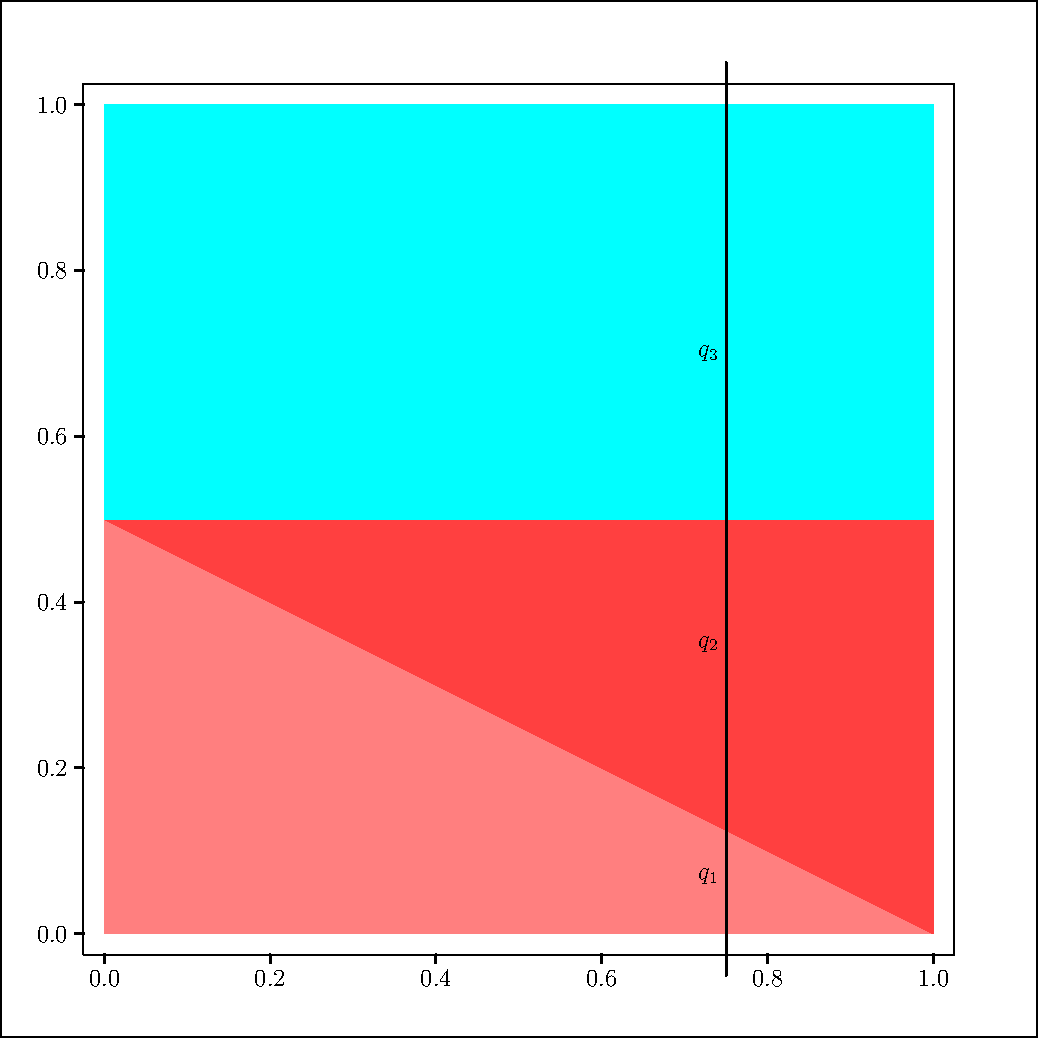
\includegraphics[width=\textwidth]{zeroone-unif.pdf}
      \caption{Judy Benjamin's posterior probability assignment
        according to intuition T1. $0<q<1$ forms the horizontal axis,
        the vertical axis shows the posterior probability distribution
        (or the normalized odds vector) $(q_{1},q_{2},q_{3})$. The
        vertical line at $q=0.75$ shows the specific posterior
        probability distribution $G_{\mbox{\tiny ind}}(0.75)$ for the Judy
        Benjamin problem.}
      \label{fig:unif}
    \end{minipage}
  \end{flushright}
\end{figure}

\begin{figure}[h]
  \begin{flushright}
    \begin{minipage}[h]{\lwv\linewidth}
      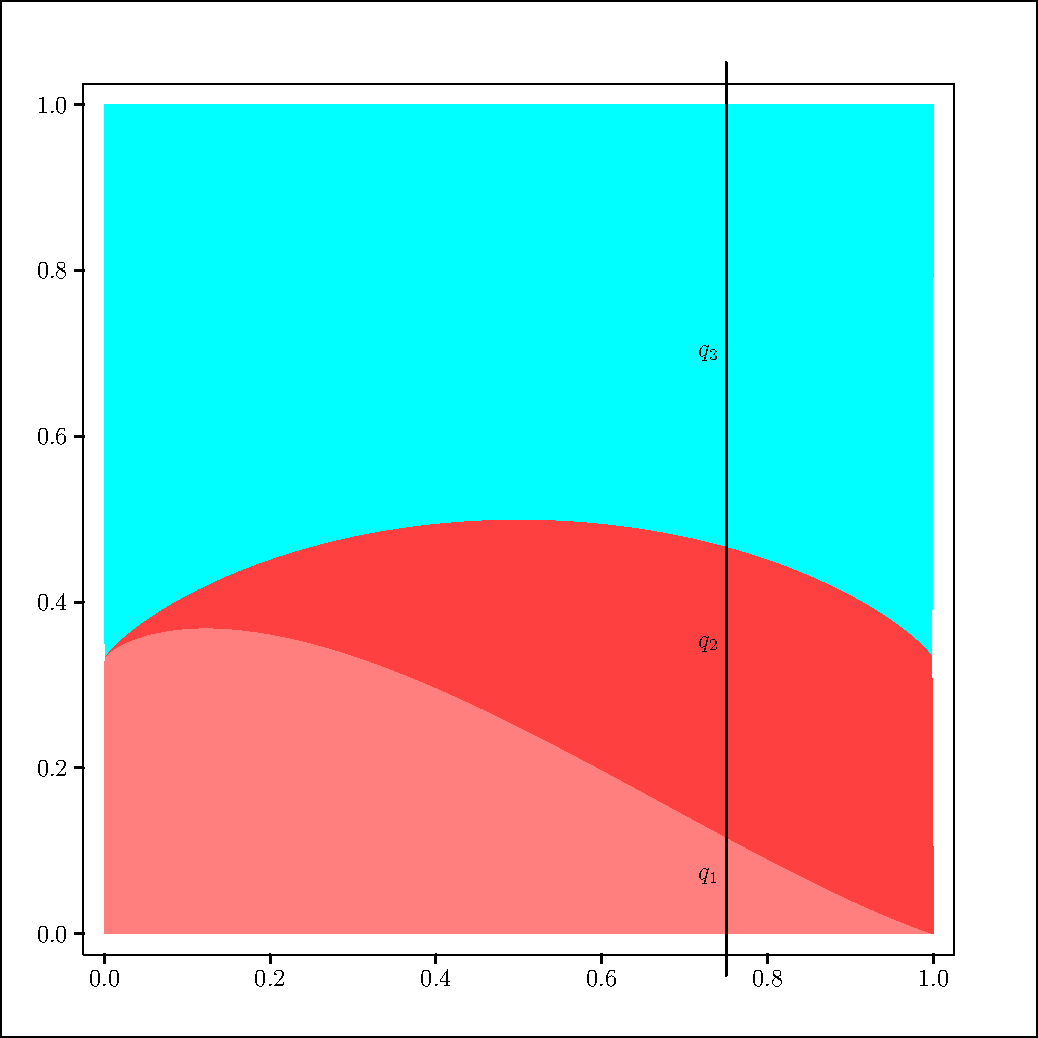
\includegraphics[width=\textwidth]{zeroone-mxnt.pdf}
      \caption{Judy Benjamin's posterior probability assignment using
        \textsc{maxent}. $0<q<1$ forms the horizontal axis, the
        vertical axis shows the posterior probability distribution (or
        the normalized odds vector) $(q_{1},q_{2},q_{3})$. The
        vertical line at $q=0.75$ shows the specific posterior
        probability distribution $G_{\mbox{\tiny max}}(0.75)$ for the Judy
        Benjamin problem.}
      \label{fig:mxnt}
    \end{minipage}
  \end{flushright}
\end{figure}

\kapt{Epistemic Entrenchment}

Even though T1 is an understandably strong intuition, it does not take
into account that the information given to Judy by her commanders may
be dependent on whether she is in Blue or in Red territory. To
underline this objection to intuition T1 we want to consider three
scenarios, any of which may form the basis of the partial information
provided by her commanders.

\begin{enumerate}
\item[\textbf{I}] Judy was dropped off by a pilot who flipped two
  coins. If the first coin landed H, then Judy was dropped off in Blue
  territory, otherwise in Red territory. If the second coin landed H,
  she was dropped off in the Headquarters area, otherwise in the
  Second Company area. Judy's commanders find out that the second coin
  was biased $q:1-q$ toward H with $q=0.75$. The normalized odds
  vector is $G_{\mbox{\tiny I}}(0.75)=(0.125,0.375,0.500)$ and agrees with T1, because the
  choice of Blue or Red is completely independent from the choice of
  the Headquarters area or the Second Company area.
\item[\textbf{II}] The pilot randomly lands in any of the four
  quadrants and rolls a die. If she rolls an even number, she drops
  off Judy. If not, she takes her to another (or the same, the choice
  happens with replacement) randomly selected quadrant to repeat the
  procedure. Judy's commanders find out, however, that for $A_{1}$,
  the pilot requires a six to drop off Judy, not just an even number.
  The normalized odds vector in this scenario is $G_{\mbox{\tiny
      II}}(0.75)=(0.1,0.3,0.6)$ and does not accord with T1.
\item[\textbf{III}] Judy's commanders have divided the map into $24$
  congruent rectangles, $A_{3}$ into twelve, and $A_{1}$ and $A_{2}$
  into six rectangles each (see figures~\ref{fig:pwstex1} and
  \ref{fig:pwstex2}). They have information that the only subsets of
  the $24$ rectangles in which Judy Benjamin may be located are such
  that they contain three times as many $A_{2}$ rectangles than
  $A_{1}$ rectangles. The normalized odds vector in this scenario is
  $G_{\mbox{\tiny III}}(0.75)\approx(.108,.324,.568)$ (evaluating almost
  17 million subsets).
\end{enumerate}

I--III demonstrate the contrast between scenarios when independence is
true and when it is not. Douven and Romeijn's capital mistake in their
paper is that they assume that the Judy Benjamin problem is analogous
to their example of Sarah and the sundowners at the Westcliff (see
\scite{8}{douvenromeijn09}{7}). Sarah, however, knows that whether it
rains or not is independent of her activity the next night, whereas in
Judy Benjamin we have no evidence of such independence, as scenario II
demonstrates. Douven and Romeijn's reliance on intuition T1 leads them
to apply Jeffrey's rule to the Judy Benjamin problem with the
additional constraint $Q(A_{3})=P(A_{3})$. They claim that in most
cases \qeins{the learning of a conditional is or would be irrelevant
  to one's degree of belief for the conditional's antecedent {\ldots}
  the learning of the relevant conditional should intuitively leave
  the probability of the antecedent unaltered}
\scite{2}{douvenromeijn09}{9}. This, according to Douven and Romeijn,
is the usual epistemic entrenchment and applies in full force to the
Judy Benjamin problem. They give an example where the epistemic
entrenchment could go the other way and leave the consequent rather
than the antecedent unaltered (Kate and Henry, see
\scite{8}{douvenromeijn09}{13}). 

Consider a 1000 ticket lottery with one winner (table below,
\textbf{[A]}) to demonstrate the role of epistemic entrenchment.
You receive the information that ticket holder X's ticket is 1000
times more likely to win than ticket holder Y's ticket (let Z be
one of the 998 other players). You consider this information
completely reliable, but you have no idea what the reasons behind
it are. The reasons may have nothing to do with X's increased
odds, but only with Y's decreased odds (table below,
\textbf{[B]}). Y's original 1/10th percent chance to win should be
evenly distributed among all participants (leaving enough for Y to
have 1/1000th of the chance to win as everybody else, including
X). Alternatively, X may have claim to all the spoils from Y while
everyone else is left alone (table below, \textbf{[C]}) . This is
analogous to Douven and Romeijn's (or Grove and Halpern's)
solution for the Judy Benjamin problem: everybody stays at odds of
1/10th of a percent except X, who will have almost 2/10ths, and Y,
who will have 1/1000th of that. There is another plausible
alternative that the information is not about Y's decreased odds
at all but about X's increased odds (table below, \textbf{[D]}) .
Then X's odds of winning the lottery are slightly more than 1/2,
while Y and the other 998 players share the other half. Following
the constraint rule, \textsc{maxent} gives X roughly eight times
more of Y's share than everyone else, but comparatively X does not
gain much (table below, \textbf{[E]}). \textsc{maxent}
approximately hands Y 1/1000th of its original share, X 8/1000th,
and everybody else 991/1000th (for each individual, this is
divided by 998). Douven and Romeijn would say that \textsc{maxent}
commits itself to something that is better left in the hands of an
epistemic entrenchment. The following table shows how these
epistemic entrenchments make a big difference in the posterior
probability distribution (expressed in 1/10ths of a percent), and
how they can put \textsc{maxent} on the spot to make decisions
that may appear overcommitted (\textbf{[B]} and \textbf{[E]} are
similar enough to suggest that \textsc{maxent} supports
\textbf{[B]}).

\begin{tabular}{|l|r|r|r|r|}\hline
& $P(X)$ & $P(Y)$ & $P(Z)$ \\ \hline
\textbf{[A]}& \texttt{1.000000000} & \texttt{1.000000000} & \texttt{1.000000000} \\ \hline
\textbf{[B]}& \texttt{1.000999999} & \texttt{0.001000999} & \texttt{1.000999999} \\ \hline
\textbf{[C]}& \texttt{1.998001998} & \texttt{0.001998002} & \texttt{1.000000000} \\ \hline
\textbf{[D]}& \texttt{500.250125063} & \texttt{0.500250125} & \texttt{0.500250125} \\ \hline
\textbf{[E]}& \texttt{1.007924650} & \texttt{0.001007925} & \texttt{1.000993054} \\ \hline
\end{tabular}

Using Hellinger's distance, an epistemic entrenchment could settle
anywhere in the middle between the two extremes \qnull{don't touch
  the antecedent} and \qnull{don't touch the consequent}. Similar
to R{\'e}nyi entropies, this leads to what Carnap might have
called a continuum of inductive methods, but more to the point it
leads to the full employment theorem in probability kinematics
discussed above: the art of judgment on part of the human inquirer
receives the limelight rather than a method which severely
constrains the inquirer's room for choice.

\kapt{The Powerset Approach}

In this section, we will focus on scenario III and consider what
happens when the grain of the partition becomes finer. We call
this the powerset approach. Two remarks are in order: (1) The
powerset approach has little independent appeal. The reason behind
using \textsc{maxent} is that we want our evidence to have just
the right influence on our posterior probabilities, i.e.\ neither
over-inform nor under-inform. There is no corresponding reason why
we should update our probabilities using the powerset approach.

(2) What the powerset approach does is lend support to another
approach. In this task, it is persuasive because it tells us what
would happen if we were to divide the event space into infinitesimally
small, uniformly weighed, and independent \qnull{atomic} bits of
information. It would be especially interesting if the powerset
approach did not support the independence and uniformity assumptions
of intuition T1, because both of these features are strongly
represented in the powerset approach.

Let's assume a partition $\{B_{i}\}_{i=1,{\ldots},4n}$ of
$A_{1}\cup{}A_{2}\cup{}A_{3}$ into sets that are of equal measure
$\mu$ and whose intersection with $A_{i}$ is either the empty set or
the whole set itself (this is the division into rectangles of scenario
III). ({\ref{eq:map}}) dictates that the number of sets covering $A_{3}$ equals
the number of sets covering $A_{1}\cup{}A_{2}$. For convenience, we
assume the number of sets covering $A_{1}$ to be $n$. Let
$\mathcal{C}$, a subset of the powerset of
$\{B_{i}\}_{i=1,{\ldots},4n}$, be the collection of sets which agree
with the constraint imposed by ({\ref{eq:hdq}}), i.e.\
\begin{displaymath}
  C\in\mathcal{C}\mbox{ iff }C=\{C_{j}\}\mbox{ and }t\mu\left(\bigcup{}C_{j}\cap{}A_{1}\right)=\mu\left(\bigcup{}C_{j}\cap{}A_{2}\right)
\end{displaymath}
In figures~\ref{fig:pwstex1} and \ref{fig:pwstex2} there are diagrams
of two elements of the powerset of $\{B_{i}\}_{i=1,{\ldots},4n}$. One
of them (figure~\ref{fig:pwstex1}) is not a member of $\mathcal{C}$,
the other one (figure~\ref{fig:pwstex2}) is. 

\begin{figure}[h]
  \begin{flushright}
    \begin{minipage}[h]{\lwv\linewidth}
      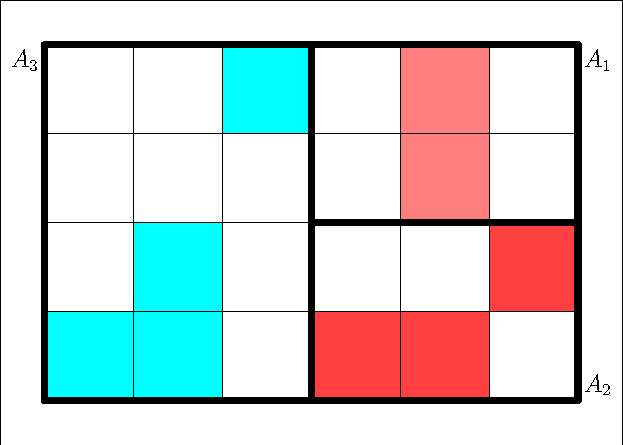
\includegraphics[width=\textwidth]{partition-2.pdf}
      \caption{This choice of rectangles is not a member of
        $\mathcal{C}$ because the number of rectangles in $A_{2}$ is
        not a $t$-multiple of the number of rectangles in $A_{1}$,
        here with $s=2,t=3$ as in scenario III.}
      \label{fig:pwstex1}
    \end{minipage}
  \end{flushright}
\end{figure}

\begin{figure}[h]
  \begin{flushright}
    \begin{minipage}[h]{\lwv\linewidth}
      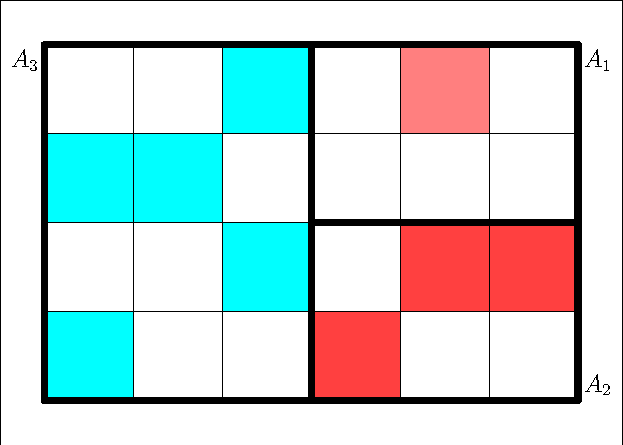
\includegraphics[width=\textwidth]{partition-1.pdf}
      \caption{This choice of rectangles is a member of
        $\mathcal{C}$ because the number of rectangles in $A_{2}$ is
        a $t$-multiple of the number of rectangles in $A_{1}$,
        here with $s=2,t=3$ as in scenario III.}
      \label{fig:pwstex2}
    \end{minipage}
  \end{flushright}
\end{figure}

Let $X$ be the random variable that corresponds to the ratio of the
number of partition elements (rectangles) that are in $A_{3}$ and the
total number of partition elements (rectangles) for a randomly chosen
$C\in\mathcal{C}$. We would now anticipate that the expectation of $X$
(which we will call $EX$) gives us an indication of the posterior
probability that Judy is in $A_{3}$ (so $EX\approx{}q_{3}$). The powerset
approach is often superior to the uniformity approach (Grove and
Halpern use uniformity, with all the necessary qualifications): if you
have played Monopoly, you will know that the frequencies for rolling a
2, a 7, or a 10 with two dice tend to conform more closely to the
binomial distribution (based on a powerset approach) rather than to
the uniform distribution with $P(\mbox{rolling }i)=1/11$ for
$i=2,{\ldots},12$.

The binomial distribution dictates the value of $EX$, using simple
combinatorics. In this case we require, again for convenience, that
$n$ be divisible by $t$ and the \qnull{grain} of the partition $A$ be
$s=n/t$. We introduce a few variables which later on will help for
abbreviation:
\begin{displaymath}
n=ts\hspace{.5in}
2m=n\hspace{.5in}
2j=n-1\hspace{.5in}
{T}=t^{2}+1
\end{displaymath}
$EX$, of course, depends both on the grain of $A$ and the value of
$t$. It makes sense to make it independent of the grain by letting the
grain become increasingly finer and by determining $EX$ as
$s\rightarrow\infty$. This cannot be done for the binomial
distribution, as it is notoriously uncomputable for large numbers
(even with a powerful computer things get dicey around $s=10$). But,
equally notorious, the normal distribution provides a good
approximation of the binomial distribution and will help us arrive at
a formula for $G_{\mbox{\tiny pws}}$ (corresponding to 
$G_{\mbox{\tiny ind}}$ and $G_{\mbox{\tiny max}}$), determining the value $q_{3}$
dependent on $q$ as suggested by the powerset approach.

First, we express the random variable $X$ by the two independent
random variables $X_{12}$ and $X_{3}$. $X_{12}$ is the number of
partition elements in the randomly chosen $C$ which are either in
$A_{1}$ or in $A_{2}$ (the random variable of the number of partition
elements in $A_{1}$ and the random variable of the number of partition
elements in $A_{2}$ are decisively not independent, because they need
to obey ({\ref{eq:hdq}})); $X_{3}$ is the number of partition elements
in the randomly chosen $C$ which are in $A_{3}$. A relatively simple
calculation shows that $EX_{3}=n$, which is just what we would expect
(either the powerset approach or the uniformity approach would give us
this result):
\begin{displaymath}
  EX_{3}=2^{-2n}\sum_{i=0}^{2n}i\binom{2n}{i}=n\mbox{ (use }\binom{n}{k}=\frac{n}{k}\binom{n-1}{k-1}\mbox{)}
\end{displaymath}

The expectation of $X$, $X$ being the random variable expressing the
ratio of the number of sets covering $A_{3}$ and the number of sets
covering $A_{1}\cup{}A_{2}\cup{}A_{3}$, is
\begin{displaymath}
  EX=\frac{EX_{3}}{EX_{12}+EX_{3}}=\frac{n}{EX_{12}+n}
\end{displaymath}
If we were able to use uniformity and independence, $EX_{12}=n$ and
$EX=1/2$, just as Grove and Halpern suggest (although their uniformity
approach is admittedly less crude than the one used here). Will the
powerset approach concur with the uniformity approach, will it support
the principle of maximum entropy, or will it make another suggestion
on how to update the prior probabilities? To answer this question, we
must find out what $EX_{12}$ is, for a given value $t$ and
$s\rightarrow\infty$, using the binomial distribution and its
approximation by the normal distribution.

Using combinatorics,
\begin{displaymath}
  EX_{12}=(t+1)\frac{\sum_{i=1}^{s}i\binom{ts}{i}\binom{ts}{ti}}{\sum_{i=0}^{s}\binom{ts}{i}\binom{ts}{ti}}
\end{displaymath}

Let us call the numerator of this fraction NUM and the denominator
DEN. According to the de Moivre-Laplace Theorem,
\begin{displaymath}
  \mbox{DEN}=\sum_{i=0}^{s}\binom{ts}{i}\binom{ts}{ti}\approx{}2^{2n}\sum_{i=0}^{s}\int_{i-\frac{1}{2}}^{i+\frac{1}{2}}\mathcal{N}(\frac{n}{2},\frac{n}{4})(i)\mathcal{N}(\frac{n}{2},\frac{n}{4})(ti)di
\end{displaymath}
where
\begin{displaymath}
  \mathcal{N}(\mu,\sigma^{2})(x)=\frac{1}{\sqrt{2\pi\sigma^{2}}}\exp\left(-\frac{(x-\mu)^{2}}{2\sigma^{2}}\right)
\end{displaymath}
Substitution yields
\begin{displaymath}
  \mbox{DEN}\approx{}2^{2n}\frac{1}{\pi{}m}\sum_{i=0}^{s}\int_{i-\frac{1}{2}}^{i+\frac{1}{2}}\exp\left(-\frac{\left(x-m\right)^{2}}{m}-\frac{t^{2}\left(x-\frac{m}{t}\right)^{2}}{m}\right)dx
\end{displaymath}
Consider briefly the argument of the exponential function:
\begin{displaymath}
  -\frac{\left(x-m\right)^{2}}{m}-\frac{t^{2}\left(x-\frac{m}{t}\right)^{2}}{m}=-\frac{t^{2}}{m}({\aden}x^{2}+{\bden}x+{\cden})=-\frac{t^{2}}{m}\left({\aden}(x-{\hden})^{2}+{\kden}\right)
\end{displaymath}
with (the double prime sign corresponds to the simple prime sign for
the numerator later on)
\begin{displaymath}
{\aden}=\frac{1}{t^{2}}{T}\notag\hspace{.5in}
{\bden}=(-2m)\frac{1}{t^{2}}(t+1)\hspace{.5in}
{\cden}=2m^{2}\frac{1}{t^{2}}
\end{displaymath}
\begin{displaymath}
{\hden}=-{\bden}/2{\aden}\hspace{.5in}
{\kden}={\aden}{\hden}^{2}+{\bden}{\hden}+{\cden}
\end{displaymath}
Consequently,
\begin{displaymath}
\mbox{DEN}\approx{}2^{2n}\exp\left(-\frac{t^{2}}{m}{\kden}\right)\sqrt{\frac{1}{\pi{}{\aden}mt^{2}}}\int_{-\infty}^{s+\frac{1}{2}}\mathcal{N}\left({\hden},\frac{m}{2{\aden}t^{2}}\right)dx
\end{displaymath}
And, using the error function for the cumulative density function of
the normal distribution,
\begin{equation}
  \label{eq:den}
  \mbox{DEN}\approx{}2^{2n-1}\sqrt{\frac{1}{\pi{}{\aden}mt^{2}}}\exp\left(-\frac{{\kden}t^{2}}{m}\right)\left(1-\erf({\wden})\right)
\end{equation}
with
\begin{displaymath}
  {\wden}=\frac{t\sqrt{{\aden}}\left(s+\frac{1}{2}-{\hden}\right)}{\sqrt{m}}
\end{displaymath}

We proceed likewise with the numerator, although the additional factor
introduces a small complication:
  \begin{eqnarray*}
  \mbox{NUM}&=&\sum_{i=1}^{s}i\binom{ts}{i}\binom{ts}{ti}=\sum_{i=1}^{s}s\binom{ts}{i}\binom{ts-1}{ti-1}\\
&\approx&s2^{2n-1}\sum_{i=1}^{s}\mathcal{N}\left(m,\frac{m}{2}\right)(i)\mathcal{N}\left(j,\frac{j}{2}\right)(ti-1)
\end{eqnarray*}
Again, we substitute and get
\begin{displaymath}
  \mbox{NUM}\approx{}s2^{2n-1}\left(\pi\sqrt{mj}\right)^{-1}\sum_{0}^{s-1}\int_{i-\frac{1}{2}}^{i+\frac{1}{2}}\exp\left({\anum}(x-{\hnum})^{2}+{\knum}\right)
\end{displaymath}
where the argument for the exponential function is
\begin{displaymath}
  -\frac{1}{mj}\left(j(x-m)^{2}+mt^{2}\left(x-\frac{j+1}{t}\right)^{2}\right)
\end{displaymath}
and therefore
\begin{displaymath}
{\anum}=j+mt^{2}\hspace{.5in}
{\bnum}=2j(1-m)+2mt\left(t-j\right)\hspace{.5in}
{\cnum}=j(1-m)^{2}+m\left(t-j-1\right)^{2}
\end{displaymath}
\begin{displaymath}
{\hnum}=-{\bnum}/2{\anum}\hspace{.5in}
{\knum}={\anum}{\hnum}^{2}+{\bnum}{\hnum}+{\cnum}
\end{displaymath}
Using the error function, 
\begin{equation}
  \label{eq:num}
  \mbox{NUM}\approx{}2^{2n-2}\frac{s}{\sqrt{\pi{}{\anum}}}\exp\left(-\frac{{\knum}}{mj}\right)\left(1+\erf({\wnum})\right)
\end{equation}
with
\begin{displaymath}
  {\wnum}=\frac{\sqrt{{\anum}}\left(s-\frac{1}{2}-{\hnum}\right)}{\sqrt{mj}}
\end{displaymath}

Combining ({\ref{eq:den}}) and ({\ref{eq:num}}),
\begin{eqnarray*}
  EX_{12}&=&(t+1)\frac{\mbox{NUM}}{\mbox{DEN}}\\
&\approx&\frac{1}{2}(t+1)\sqrt{\frac{{T}{}ts}{{T}{}ts-1}}se^{\alpha_{t,s}}
\end{eqnarray*}
for large $s$, because the arguments for the error function $w'$ and
$w''$ escape to positive infinity in both cases (NUM and DEN) so that
their ratio goes to 1. The argument for the exponential function is
\begin{displaymath}
  \alpha_{t,s}=-\frac{{\knum}}{mj}+\frac{{\kden}t^{2}}{m}
\end{displaymath}
and, for $s\rightarrow\infty$, goes to
\begin{displaymath}
  \alpha_{t}=\frac{1}{2}{T}^{-2}(2t^{3}-3t^{2}+4t-5)
\end{displaymath}

Notice that, for $t\rightarrow\infty$, $\alpha_{t}$ goes to $0$ and
\begin{displaymath}
  EX=\frac{n}{EX_{12}+n}\rightarrow\frac{2}{3}
\end{displaymath}
in accordance with intuition T2.

We now have a formula for the powerset approach corresponding to the
formula for the \textsc{maxent} approach, giving us $q_{3}$ dependent
on $t$. Notice that this formula is for $t=2,3,4,\ldots$. For $t=1$
use the Chu-Vandermonde identity to find that
\begin{displaymath}
  EX_{12}=(t+1)\frac{\sum_{i=1}^{s}i\binom{ts}{i}\binom{ts}{ti}}{\sum_{i=0}^{s}\binom{ts}{i}\binom{ts}{ti}}=(t+1)\frac{s}{2}  
\end{displaymath}
and consequently $EX=1/2$, as one would expect. For
$t=1/2,1/3,1/4,\ldots$ we can simply reverse the roles of $A_{1}$ and
$A_{2}$. These results give us $G_{\mbox{\tiny pws}}$ and a graph of
the normalized odds vector (see figure~\ref{fig:pwst}), a bit bumpy
around the middle because the $t$-values are discrete and farther
apart in the middle, as $t=q/(1-q)$. Comparing the graphs of the
normalized odds vector under Grove and Halpern's uniformity approach
($G_{\mbox{\tiny ind}}$), Jaynes' \textsc{maxent} approach
($G_{\mbox{\tiny max}}$), and the powerset approach suggested in this
paper ($G_{\mbox{\tiny pws}}$), it is clear that the powerset approach
supports \textsc{maxent}.

\begin{figure}[h]
  \begin{flushright}
    \begin{minipage}[h]{\lwv\linewidth}
      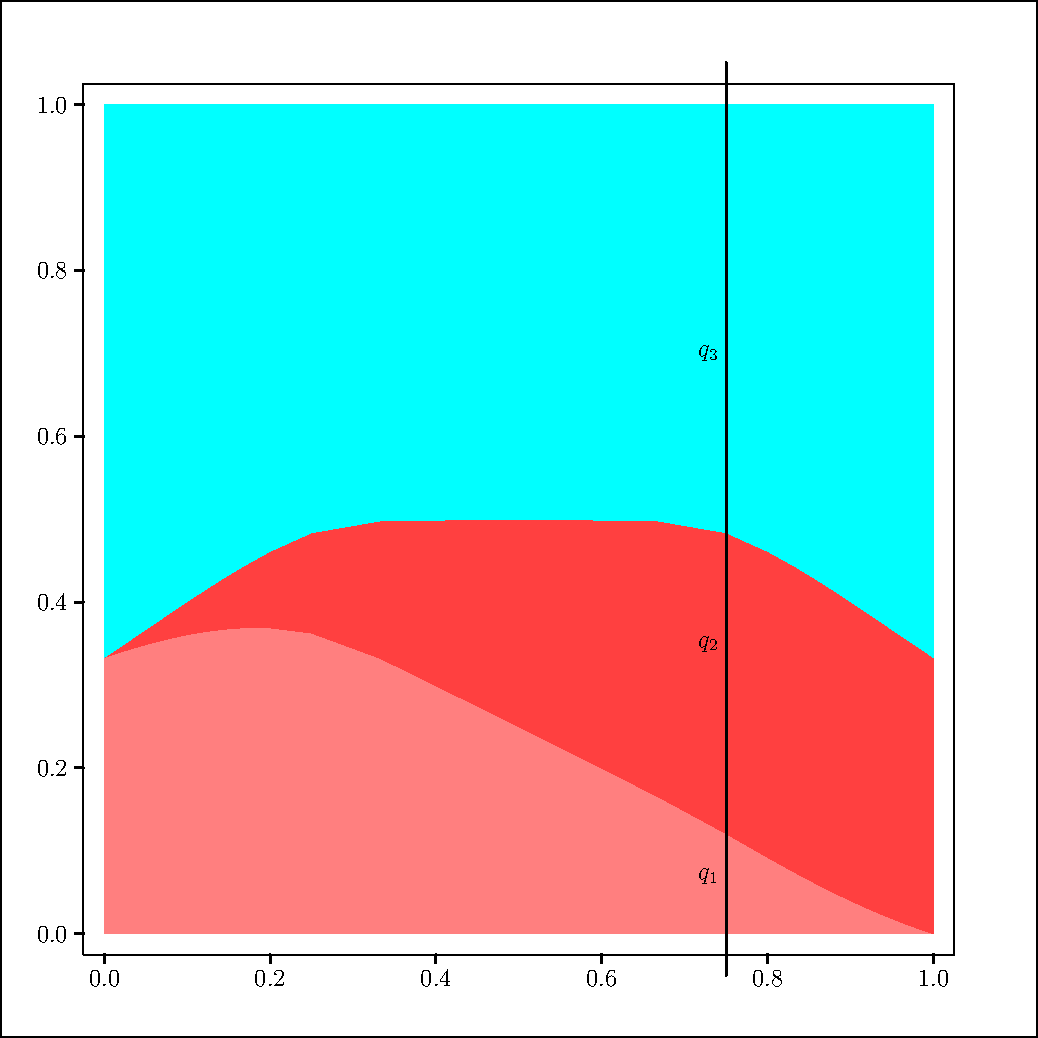
\includegraphics[width=\textwidth]{zeroone-pwst.pdf}
      \caption{Judy Benjamin's posterior probability assignment
        according to the powerset approach. $0<q<1$ forms the
        horizontal axis, the vertical axis shows the posterior
        probability distribution (or the normalized odds vector)
        $(q_{1},q_{2},q_{3})$. The vertical line at $q=0.75$ shows the
        specific posterior probability distribution $G_{\mbox{\tiny
            pws}}$ for the Judy Benjamin problem.}
      \label{fig:pwst}
    \end{minipage}
  \end{flushright}
\end{figure}

% analogous to the way in which the normal distribution captures so
% many natural phenomena because it generalizes the binomial
% distribution with its discrete on/off switches (as in a Galton box) to
% an infinite grain and a smooth distribution.

Going through the calculations, it seems at many places that the
powerset approach should give its support to Grove and Halpern's
uniformity approach in keeping with intuition T1. It was unexpected to
find out that in the mathematical analysis $\alpha_{t,s}$ converges to
a non-trivial factor and did not tend to negative or positive
infinity, enabling a graph of the normalized odds vector that was not
of the simple nature of the graph suggested by Grove and Halpern. Most
surprisingly, the powerset approach, prima facie unrelated to an
approach using information, supports the idea that a set of events
about which nothing is known (such as $A_{3}$) gains in probability in
the posterior probability distribution compared to the set of events
about which something is known (such as $A_{1}$ and $A_{2}$), even if
it is only partial information. Unless independence is specified, as
in Sarah and sundowners at the Westcliff, the area of ignorance gains
compared to the area of knowledge.

\kapt{Conclusion}

\tbd{We suggest that Seidenfeld's objection that \textsc{maxent} is
\qeins{excessively aprioristic} is a simple instance of the
well-calibrated Bayesian's problem with coherence (see
\scite{7}{dawid82}{}) and pertains to Bayesian conditionalization
methods in general.}

We now have several ways to characterize Judy's posterior
probabilities and posterior probabilities following upon partial
information in general. Only one of them, the uniformity approach,
violates van Fraassen, Hughes, and Harman's five symmetry requirements
in \scite{1}{fraassenetal86}{} and intuition T2. The uniformity
approach, however, is the only one that satisfies intuition T1, an
intuition which most people have when they first hear the story (see
Grove and Halpern \scite{7}{grovehalpern97}{} and Douven and Romeijn
\scite{7}{douvenromeijn09}{} for a strong defence of T1 even in the
face of van Fraassen and colleagues' symmetry requirements). We have
two arguments attenuating the position of the uniformity approach in
comparison with the others.

\begin{enumerate}[(1)]
\item T1 rests on an independence assumption which is not reflected in
  the problem. Although there is no indication that what Judy's
  commanders tell her is in any way dependent on her probability of
  being in Blue territory, it is not excluded either (see scenarios
  I--III earlier in this paper). \textsc{maxent} in particular takes
  this uncertainty into consideration.
\item When we investigate the problem using the powerset approach it
  turns out that a division into equally probable, independent, and
  increasingly fine bits of information supports not intuition T1 but
  rather intuition T2.
\end{enumerate}

There are other approaches that we could have thrown into the mix,
e.g.\ maximum transition probability (MTP) and van Fraassen, Hughes,
and Harman's MUD. None of them, however, have the appeal of
\textsc{maxent} in the sense that they process just the right amount
of information. MUD is the simplest updating rule obeying van
Fraassen, Hughes, and Harman's symmetry requirements. MTP has in its
favour an interesting connection to the Projection Postulate in
quantum mechanics (and also obeys the symmetry requirements). Van
Fraassen, Hughes, and Harman subject all three, \textsc{maxent}, MUD,
and MTP to two tests. On both tests \textsc{maxent} places second, not
first, and the authors conclude that the superiority of
\textsc{maxent} is merely \qeins{perceived}
\scite{2}{fraassenetal86}{462}. 

A closer examination of the tests, however, reveals that
\textsc{maxent} places second in these tests precisely because it
refuses to assign either too much or too little information to the
evidence (according to Csisz{\'a}r's theorem). In the first test, the
Learning Rate Test, MUD performs better than \textsc{maxent} (and MTP
worse) because MUD tends to exaggerate the information provided by the
evidence. In the second test, the Wavering Effect Test, MTP performs
better than \textsc{maxent} (and MUD worse) because MTP tends to
understate the information provided by the evidence. \textsc{maxent}
is framed by these tests, not out of vice, but out of virtue.

Lastly, a recurring criticism of \textsc{maxent} is its rigidity. The
objectivism that is associated with it implies that there is
\qeins{little room for an agent to subjectively choose how strongly to
  believe a proposition} \scite{2}{williamson09}{4}. Jaynes' original
ambition was that there would be no room at all. Seidenfeld considers
\textsc{maxent} \qeins{excessively aprioristic}
\scite{2}{seidenfeld79}{414}; Howson and Franklin deliver a more
general attack on all constraints on updating that go beyond Bayesian
conditionalization (see \scite{7}{howsonfranklin94}{}). Howson and
Franklin raise a valid point: there needs to be a much more detailed
discussion what exactly it is that poses these constraints. Logic does
not force us to accept them, and whether rationality does is a wide
open question. 

Seidenfeld, however, just falls prey to the well-calibrated
meteorologist's fallacy when the meteorologist entertains an
understandable modesty about her calibration performance (see
\scite{7}{dawid82}{}). Once we assign a probability to an event we do
not have the luxury of subjecting this assignment to further
uncertainty, on pain of incoherence. \textsc{maxent}'s ambitions are
in this respect no worse than the forecaster's honest attempt to
settle at any number at all, knowing that once the number is announced
there is no room for doubting oneself. There is, after all, still
plenty of room for re-partitioning the theory space, making fresh
observations, designing better experiments, and pouring over the data
one more time. That is where the full employment of science is
located.

% \noindent\textbf{Endnotes}

% \theendnotes

% \medskip

\kapt{References}

% \nocite{*} 
\bibliographystyle{stefan-2010-08-28}
\bibliography{bib-3306}

\end{document}

